MD5は誤り検出符号の一種であり, データを元に出力した128 bitの値を用いる.
主に暗号や認証, デジタル署名などで用いられている.
計算方法は, まず, 計算用バッファとして、4つの符号無し32ビット整数A、B、C、Dの初期化を行う.
初期化した値は以下の通りであり, 表記は全て16 進数で表す.

$\hspace{140pt} A = 0x67452301 \\
 \hspace{150pt} B = 0xEFCDAB89 \\
 \hspace{150pt} C = 0x98BADCFE \\
 \hspace{150pt} D = 0x10325476 \\
$

次に, MD5の出力を行うために以下の4 つの補助関数を定義する.
$xy$は,ビットに関する $x$ と $y$の $AND$ を意味する.
$x U y$は、ビットに関する $x$ と $y$ の $OR$ を意味する。
$not(x)$ は、$x$ に関する補数を意味する。
$x$ $XOR$ $y$は、ビットに関する $x$ と $y$ の $XOR$ を意味する。

$\hspace{150pt} F(x,y,z) =$ $xy$ $U$ $not(x)$ $z$ \\
$\hspace{150pt} G(x,y,z) =$ $xz$ $U$ $y$ $not(z)$ \\
$\hspace{150pt} H(x,y,z) =$ $x$ $XOR$ $y$ $XOR$ $z$ \\
$\hspace{150pt} I(x,y,z) =$ $y$ $XOR$ ($x$ $U$ $not(z)$) \\


そして, MD5を計算する入力文字列Pを用意する.
Pの文字列を全てbit列へと変換を行い, bit列の長さを一定にするためにパディングを行う.
手順を図\ref{bit}に示す.
具体的には, Pの文字列を全て2 進数へと置き換え, 1 bit目が1 でそれ以外が0である文字列Qをbの末端に付与し, 合計のbit数が512 の剰余となるようにする.
これ以降, bit列は32 bitごとに区切って16 進数へと置き換えた文字列をワード列とする.
ワード列の作成方法を図\ref{wordretu}に示す.
まず32 bitを8 bit毎に区切り, それぞれ16 進数へと置き換えたのち, 下位の文字列から順に並べる.

\begin{figure}[htbp]
 \begin{minipage}{0.5\hsize}
  \begin{center}
   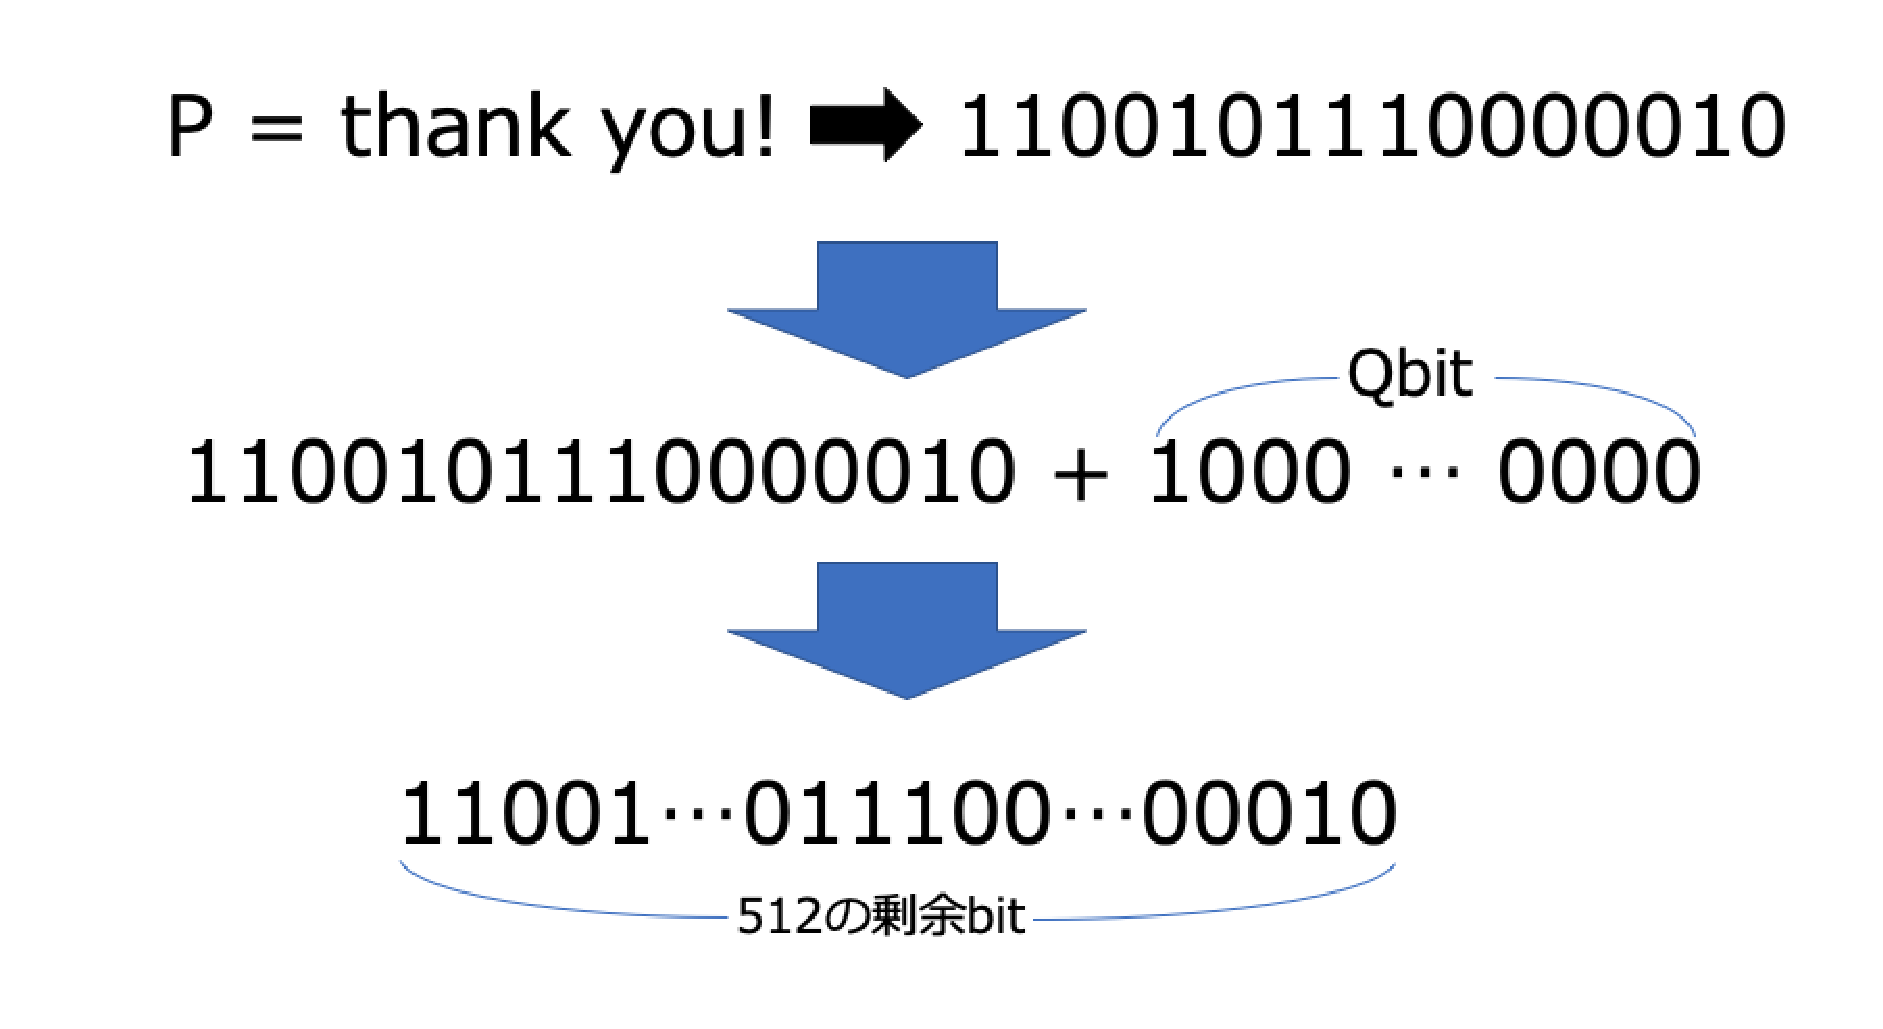
\includegraphics[width=70mm]{bitretu.eps}
  \end{center}
  \caption{bitの調整}
  \label{bit}
 \end{minipage}
 \begin{minipage}{0.5\hsize}
  \begin{center}
   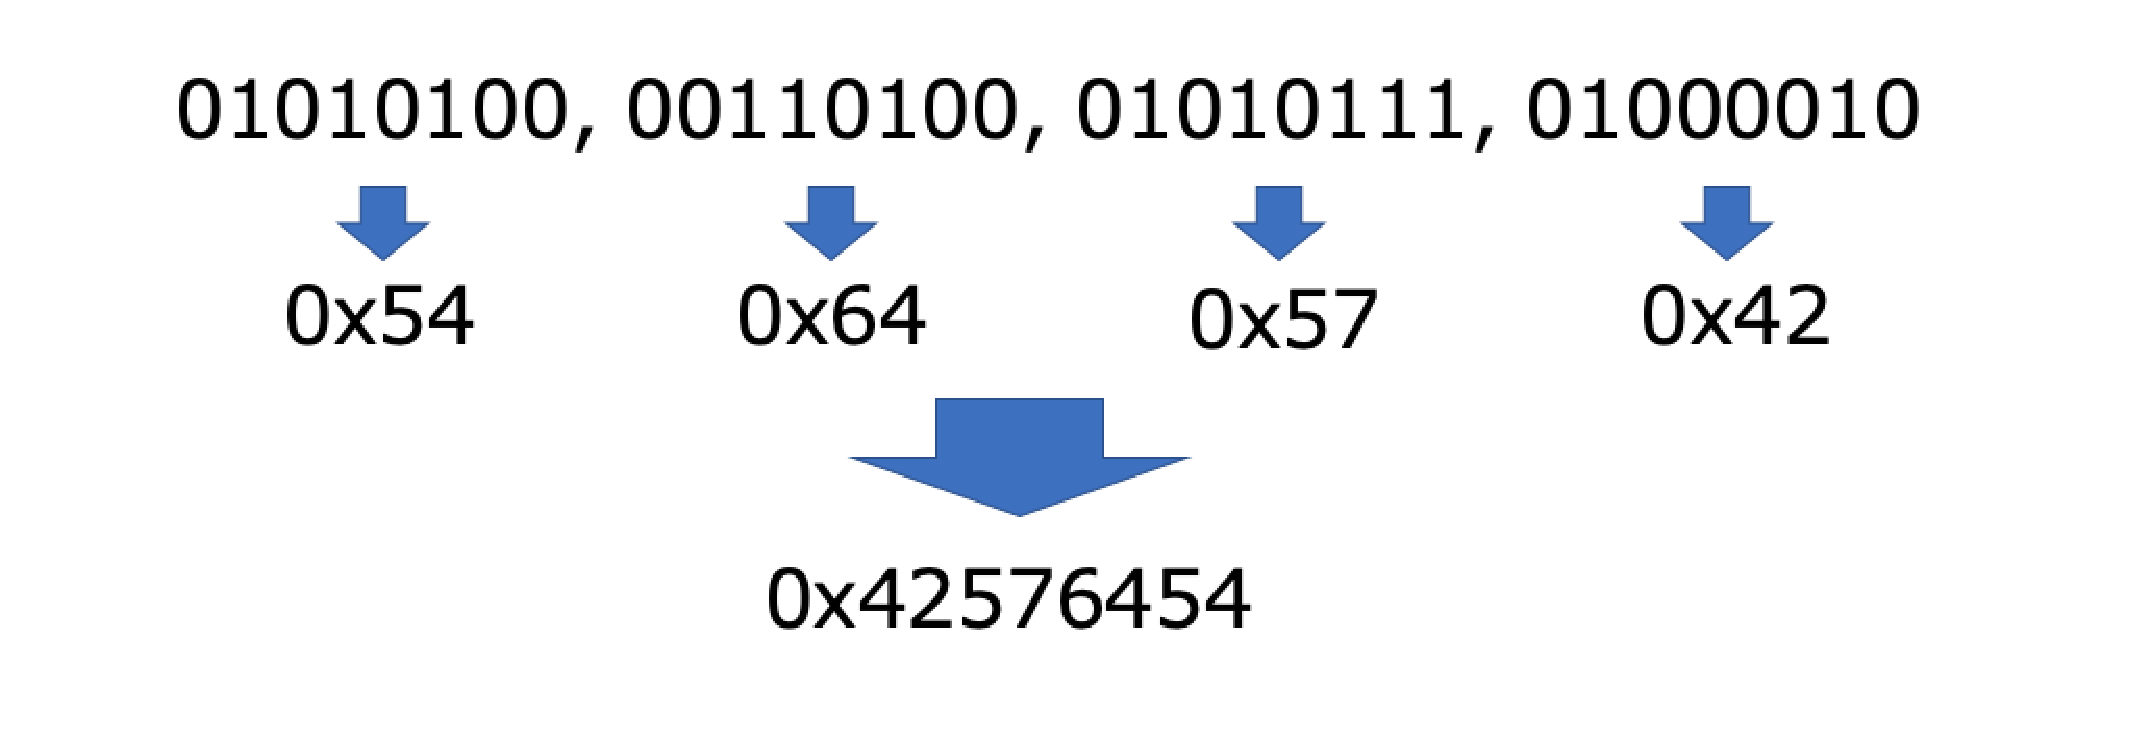
\includegraphics[width=90mm]{wordretu.eps}
  \end{center}
  \caption{ワード列}
  \label{wordretu}
 \end{minipage}
\end{figure}

次に, ワード列から取り出した16ワードを, $X0 ~ X15$の16 個の32 bit数とする. また, この時点でのバッファの値$A, B, C, D$を一時的に$A', B', C', D'$に保存する.
ここで、MD5を出力するための方程式, $Pn(abcd, k, s, i)$を以下のように定義する.
\newline

$\hspace{120pt} a = b + ((a + Fn(b, c, d) + Xk + Ti) <<< s) \\
\hspace{150pt} Tn = [2^32 |sinn|] (n = 1, 2, ...,64) \\
$

そして, 以下の処理を行い, バッファを更新する.

$P1(ABCD, 0, 7, 1); P1(DABC, 1,12, 2); P1(CDAB, 2,17, 3); P1(BCDA, 3,22, 4); \\
P1(ABCD, 4, 7, 5); P1(DABC, 5,12, 6); P1(CDAB, 6,17, 7); P1(BCDA, 7,22, 8); \\
P1(ABCD, 8, 7, 9); P1(DABC, 9,12,10); P1(CDAB,10,17,11); P1(BCDA,11,22,12); \\
P1(ABCD,12, 7,13); P1(DABC,13,12,14); P1(CDAB,14,17,15); P1(BCDA,15,22,16); \\
$
\\
$
P2(ABCD, 1, 5,17); P2(DABC, 6, 9,18); P2(CDAB,11,14,19); P2(BCDA, 0,20,20); \\
P2(ABCD, 5, 5,21); P2(DABC,10, 9,22); P2(CDAB,15,14,23); P2(BCDA, 4,20,24); \\
P2(ABCD, 9, 5,25); P2(DABC,14, 9,26); P2(CDAB, 3,14,27); P2(BCDA, 8,20,28); \\
P2(ABCD,13, 5,29); P2(DABC, 2, 9,30); P2(CDAB, 7,14,31); P2(BCDA,12,20,32); \\
$
\\
$
P3(ABCD, 5, 4,33); P3(DABC, 8,11,34); P3(CDAB,11,16,35); P3(BCDA,14,23,36); \\
P3(ABCD, 1, 4,37); P3(DABC, 4,11,38); P3(CDAB, 7,16,39); P3(BCDA,10,23,40); \\
P3(ABCD,13, 4,41); P3(DABC, 0,11,42); P3(CDAB, 3,16,43); P3(BCDA, 6,23,44); \\
P3(ABCD, 9, 4,45); P3(DABC,12,11,46); P3(CDAB,15,16,47); P3(BCDA, 2,23,48); \\
$
\\
$
P4(ABCD, 0, 6,49); P4(DABC, 7,10,50); P4(CDAB,14,15,51); P4(BCDA, 5,21,52); \\
P4(ABCD,12, 6,53); P4(DABC, 3,10,54); P4(CDAB,10,15,55); P4(BCDA, 1,21,56); \\
P4(ABCD, 8, 6,57); P4(DABC,15,10,58); P4(CDAB, 6,15,59); P4(BCDA,13,21,60); \\
P4(ABCD, 4, 6,61); P4(DABC,11,10,62); P4(CDAB, 2,15,63); P4(BCDA, 9,21,64); \\
$

最後に, 処理前のバッファの値$A', B', C', D'$と, 更新されたバッファの値$A, B, C, D$をそれぞれ加算を行い, それらを次のバッファの値$A, B, C, D$とする.
この時, ワード列にまだワードが残っているのであれば, 次の16ワードに対してくり返し上記の処理を行う.
ワード列の最後まで処理し終えたら、その時点でのバッファの値$A, B, C, D$がMD5の出力となる. \\
